\documentclass{article}[11pt]
%Required: You must have these
\usepackage{graphicx}
\usepackage{tabularx}
\usepackage{natbib}

\usepackage{array}
\usepackage{amsmath}
%\usepackage[backend=bibtex]{biblatex}
\setkeys{Gin}{width=0.8\textwidth}
%\setlength{\captionmargin}{30pt}
\setlength{\abovecaptionskip}{10pt}
\setlength{\belowcaptionskip}{10pt}
\topmargin -1.5cm 
\oddsidemargin -0.04cm 
\evensidemargin -0.04cm 
\textwidth 16.59cm
\textheight 23.94cm 
\parskip 7.2pt 
\renewcommand{\baselinestretch}{1} 	
\parindent 0pt

\bibliographystyle{refs/styles/newphyto.bst}
\renewcommand{\thetable}{S\arabic{table}}
\renewcommand{\thefigure}{S\arabic{figure}}
\usepackage{xr}
%\usepackage{hyperref}
%\usepackage{xr-hyper}
%\usepackage{hyperref}
\externaldocument{3plums_new_phyt_revisionsJan2024}


\title{Supporting Information for: Ecological drivers of flower-leaf sequences: aridity and floral traits select for flowering-first in the American Plums}
\author{D.M. Buonaiuto, T.J. Davies, S. Collins \& E.M. Wolkovich}
\date{}
\usepackage{Sweave}
\begin{document}
\input{suppliment-concordance}
\maketitle

\section*{Tables}
\begin{table}[ht]
\centering
\begin{tabular}{|lccc|}
  \hline
  species & n FLS & n petal length & n pdsi \\ 
  \hline
 alleghaniensis &  17 &  39 & 114 \\ 
americana &  95 & 271 & 200 \\ 
angustifolia &  77 & 238 & 200 \\ 
 gracilis &  85 & 289 & 200 \\ 
 hortulana & 106 & 254 & 200 \\ 
  maritima &  75 & 255 & 200 \\ 
  mexicana &  64 & 284 & 200 \\ 
  munsoniana & 117 & 279 & 200 \\ 
 nigra & 118 & 230 & 200 \\ 
   rivularis & 111 & 225 & 200 \\ 
   subcordata &  46 &  71 &  30 \\ 
   texana &  19 &  38 &  39 \\ 
  umbellata &  70 & 284 & 200 \\ 
   \hline
\end{tabular}
\caption{Sample sizes of each for each species used in this study.}
\label{tab:samps}
\end{table}

% latex table generated in R 4.1.2 by xtable 1.8-4 package
% Mon Oct  2 18:15:48 2023
% latex table generated in R 4.1.2 by xtable 1.8-4 package
% Wed Oct  4 10:01:21 2023
\begin{table}[ht]
\centering
\begin{tabular}{|lccc|}
  \hline
  species & index BBCH 0-11 & index BBCH 0-11 w/o day of season & index BBCH 0-09 \\ 
  \hline
 mexicana & 0.85 & 0.90 & 0.69 \\ 
  umbellata & 0.82 & 0.83 & 0.58 \\ 
 angustifolia & 0.76 & 0.77 & 0.51 \\ 
  maritima & 0.68 & 0.76 & 0.42 \\ 
 gracilis & 0.64 & 0.68 & 0.36 \\ 
  americana & 0.62 & 0.55 & 0.38 \\ 
  munsoniana & 0.60 & 0.67 & 0.38 \\ 
 alleghaniensis & 0.59 & 0.65 & 0.32 \\ 
  nigra & 0.55 & 0.62 & 0.30 \\ 
   hortulana & 0.51 & 0.52 & 0.28 \\ 
   texana & 0.51 & 0.54 & 0.25 \\ 
   rivularis & 0.44 & 0.53 & 0.22 \\ 
   subcordata & 0.16 & 0.18 & 0.05 \\ 
   \hline
\end{tabular}
\caption{Hysteranthy index score for 13 species in the American plums based on model predictions defining flowering during BBCH stages 0-11 as hysteranthous for models with and without day of season of observation as a covariate, and with hysteranthy defined as flowering during BBCH 0-09 only. }
\label{tab:mod1comps}
\end{table}

% xtable(fixef(mod.review.wants,probs = c(.055,.25,.75,.945)))
% latex table generated in R 4.1.2 by xtable 1.8-4 package
% Mon Oct  2 16:33:58 2023
\begin{table}[ht]
\centering
\begin{tabular}{rrccccc}
  \hline
 & Estimate & Est.Error & Q5.5 & Q25 & Q75 & Q94.5 \\ 
  \hline
Intercept & 0.34 & 0.23 & -0.02 & 0.20 & 0.48 & 0.70 \\ 
  phi\_Intercept & 1.92 & 0.42 & 1.22 & 1.65 & 2.21 & 2.55 \\ 
  pdsi.z & -0.47 & 0.30 & -0.96 & -0.66 & -0.28 & 0.01 \\ 
  petal.z & -0.14 & 0.24 & -0.54 & -0.29 & 0.01 & 0.23 \\ 
  pdsi.z:petal.z & -0.14 & 0.49 & -0.91 & -0.46 & 0.16 & 0.65 \\ 
   \hline
\end{tabular}
\end{table}
% xtable(fixef(mod.review.wants.doy,probs = c(.055,.25,.75,.945)))
% latex table generated in R 4.1.2 by xtable 1.8-4 package
% Mon Oct  2 16:34:12 2023
\begin{table}
\centering
\begin{tabular}{rrccccc}
  \hline
 & Estimate & Est.Error & Q5.5 & Q25 & Q75 & Q94.5 \\ 
  \hline
Intercept & 0.49 & 0.25 & 0.09 & 0.33 & 0.65 & 0.88 \\ 
  phi\_Intercept & 1.77 & 0.41 & 1.09 & 1.50 & 2.06 & 2.39 \\ 
  pdsi.z & -0.43 & 0.32 & -0.92 & -0.63 & -0.22 & 0.07 \\ 
  petal.z & -0.14 & 0.27 & -0.56 & -0.30 & 0.03 & 0.27 \\ 
  pdsi.z:petal.z & -0.16 & 0.54 & -1.01 & -0.50 & 0.17 & 0.69 \\ 
   \hline
\end{tabular}
\caption{Model paremeter estimates of the relationship between environmental/trait predictors and hysteranthy based on a hysteranthy index derived from a model that included day of season of observation (top table) and one that excluded this predictor from the index derivation (bottom table)}
\label{tab:nodoy}
\end{table}

\pagebreak[4]

\section*{Figures} 

\begin{figure}[h!]
    \centering
 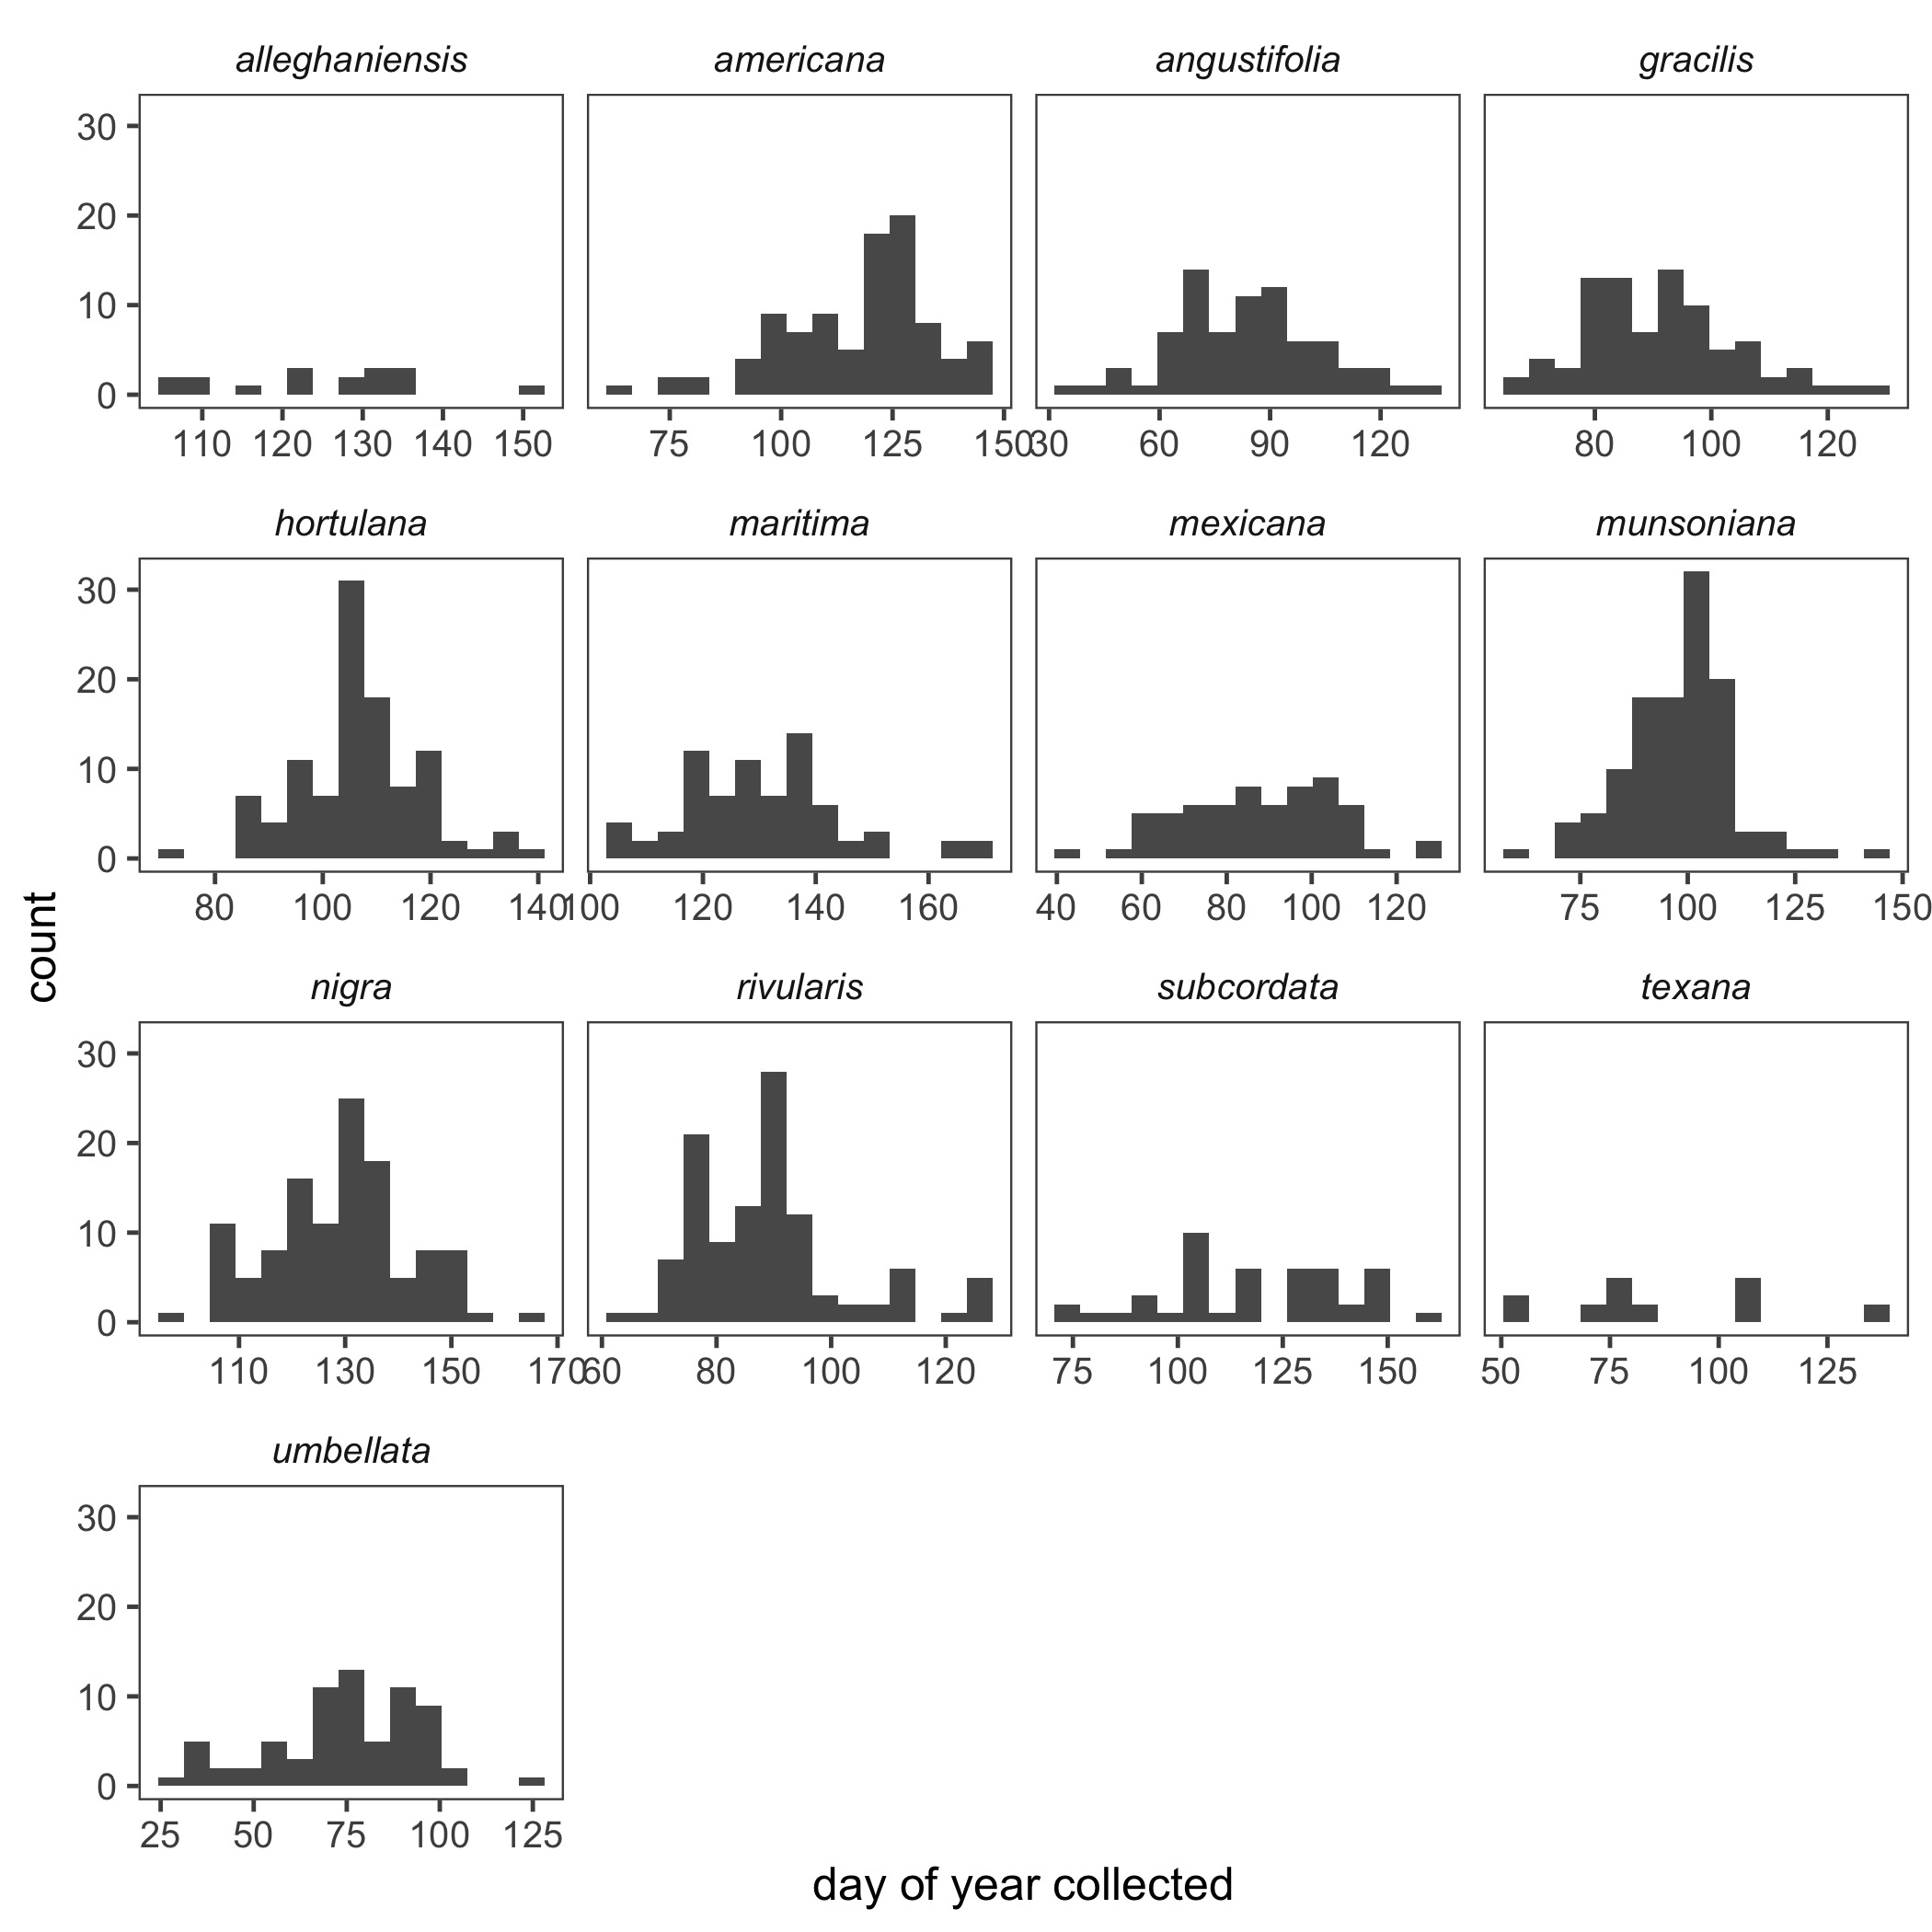
\includegraphics[width=.5\textwidth]{..//..//Plots/whatReviwerswant/seasonal_distrbn.jpeg}
   
     \caption{Histograms of collect day of year for each of the American plum species used in these analyses}
      \label{fig:bias}
\end{figure}


\begin{figure}[h!]
    \centering
 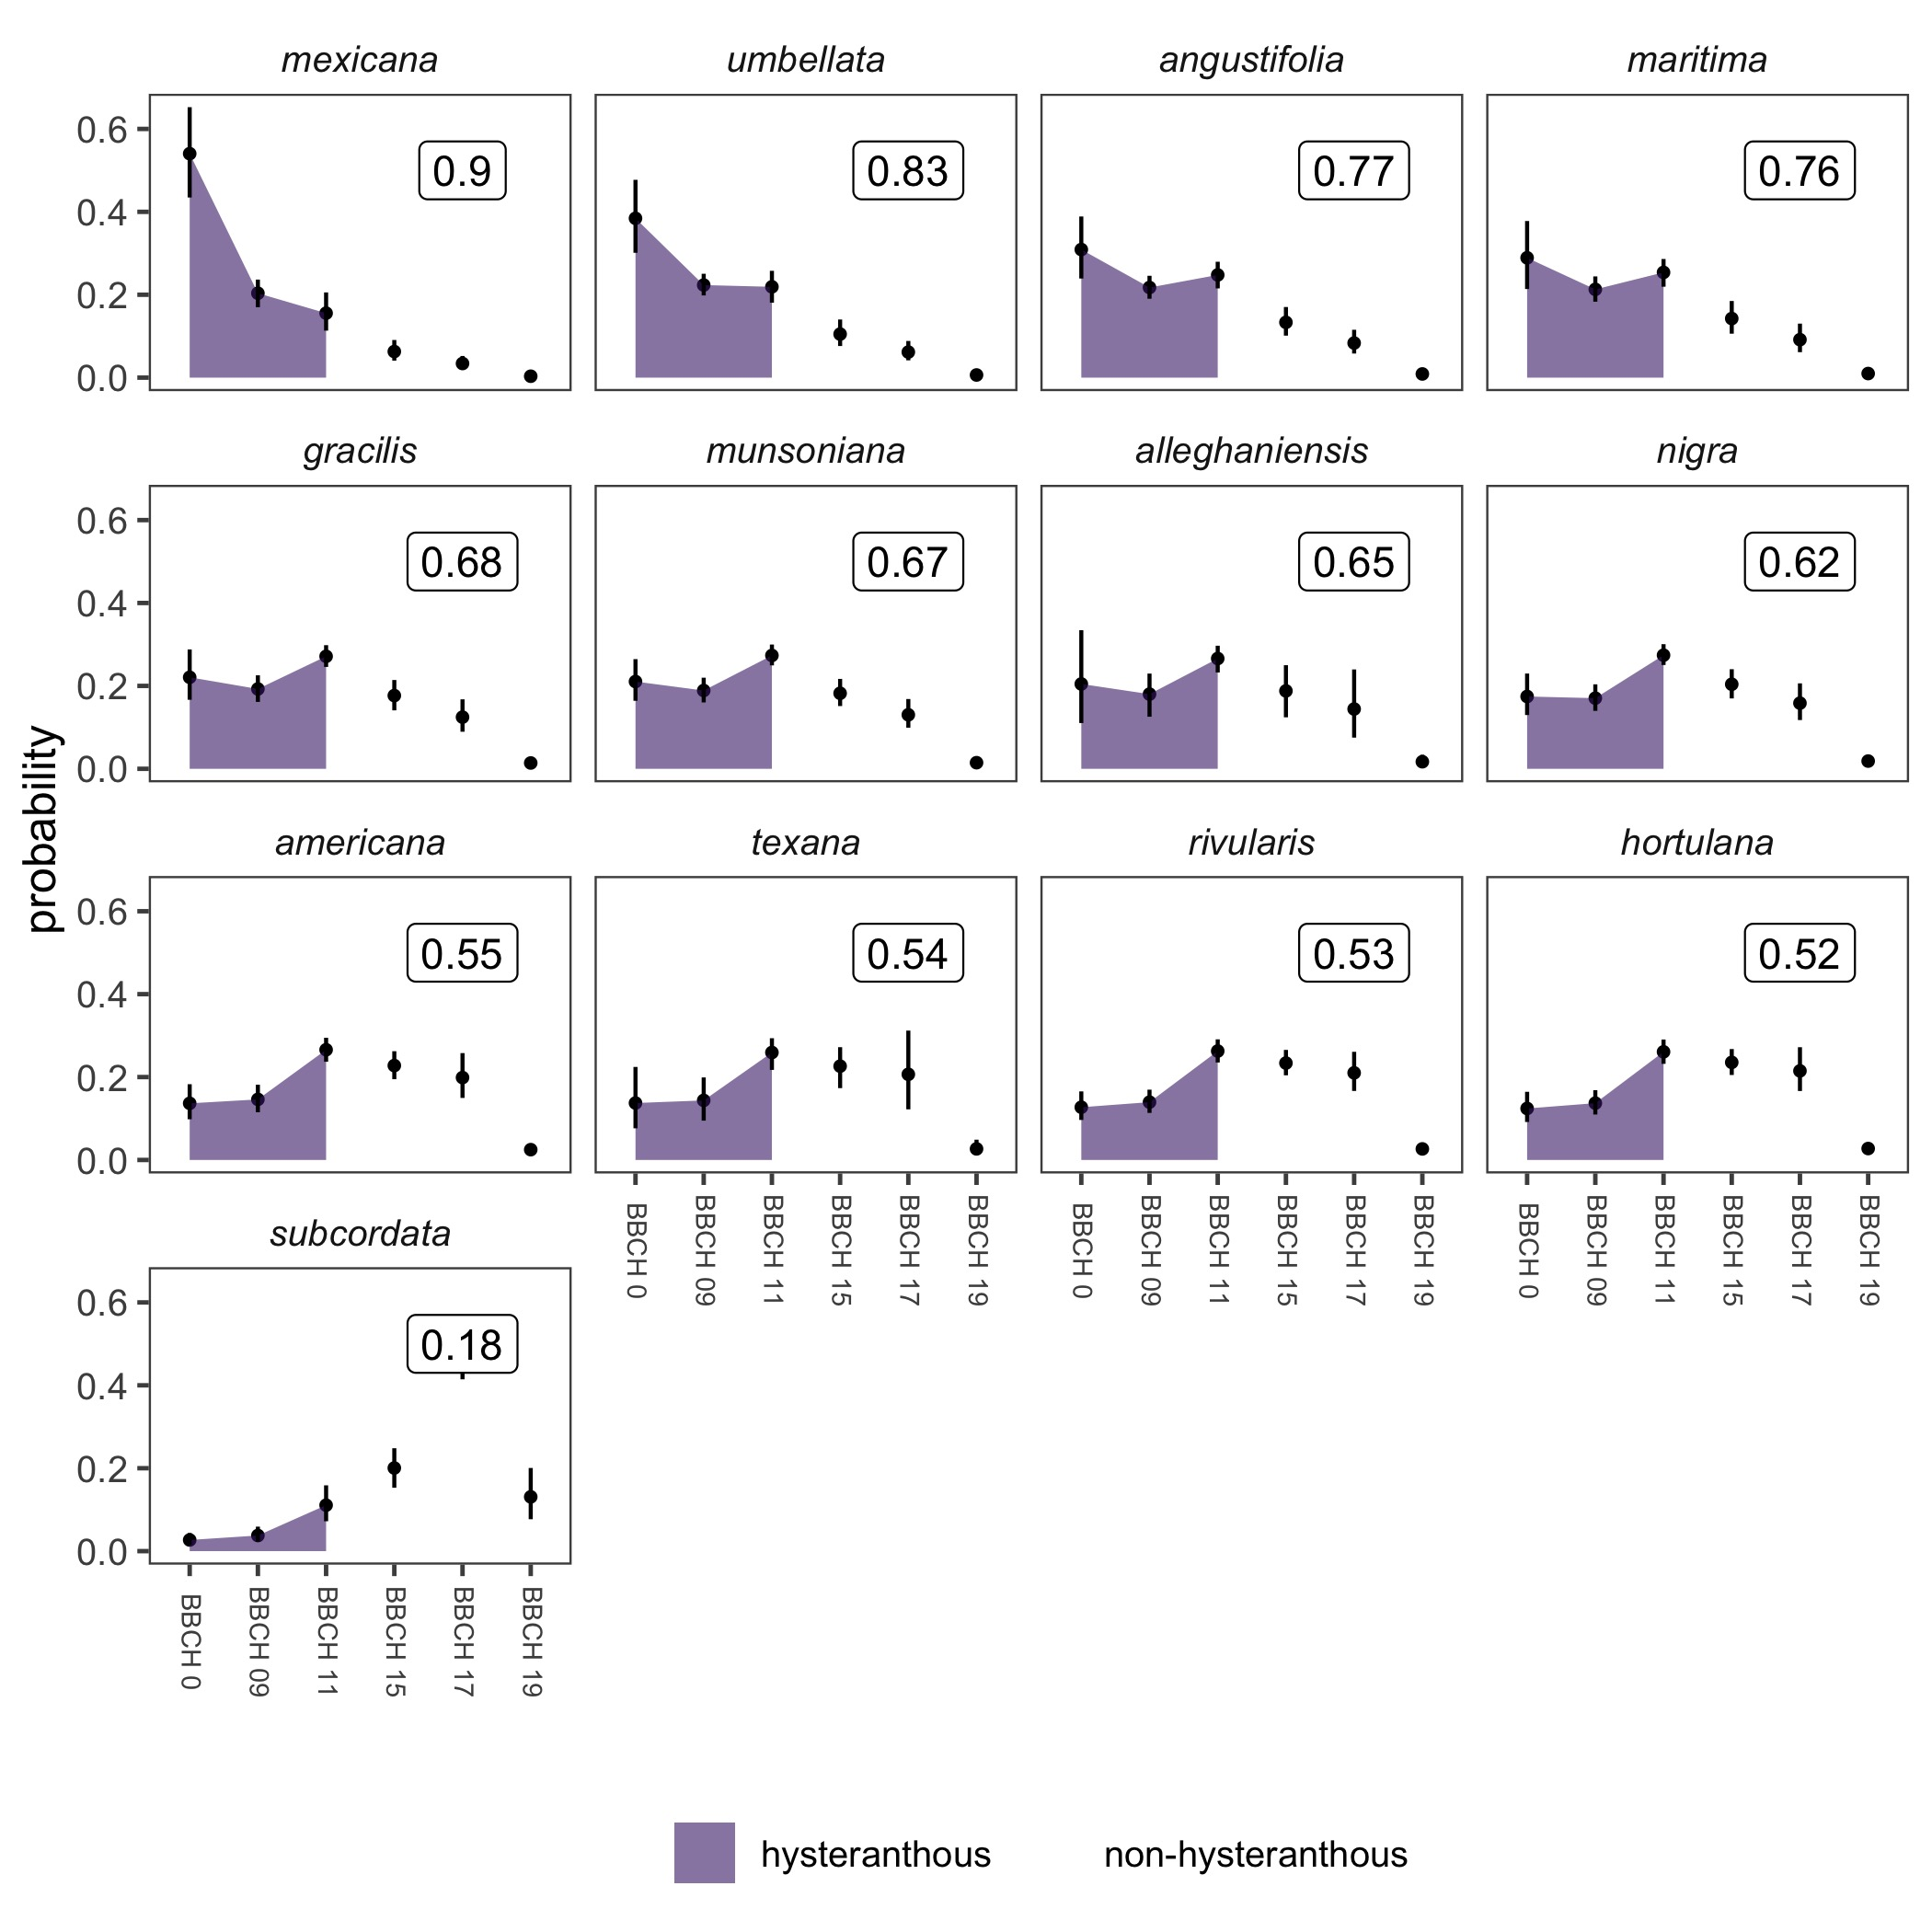
\includegraphics[width=.7\textwidth]{..//..//Plots/whatReviwerswant/sps_preds_nodoy4supp.jpeg}
    \caption{Predicted likelihood that a species would be in flower during each vegetative BBCH phase for each species in the American plums. Points are the mean likelihood while bars represent 89\% uncertainty intervals. Hysteranthy index values in each box were derived from the summed likelihood  species would be found at BBCH stages 0-11 (purple fill).}
    \label{fig:nodoy}
\end{figure}

\begin{figure}[h!]
    \centering
 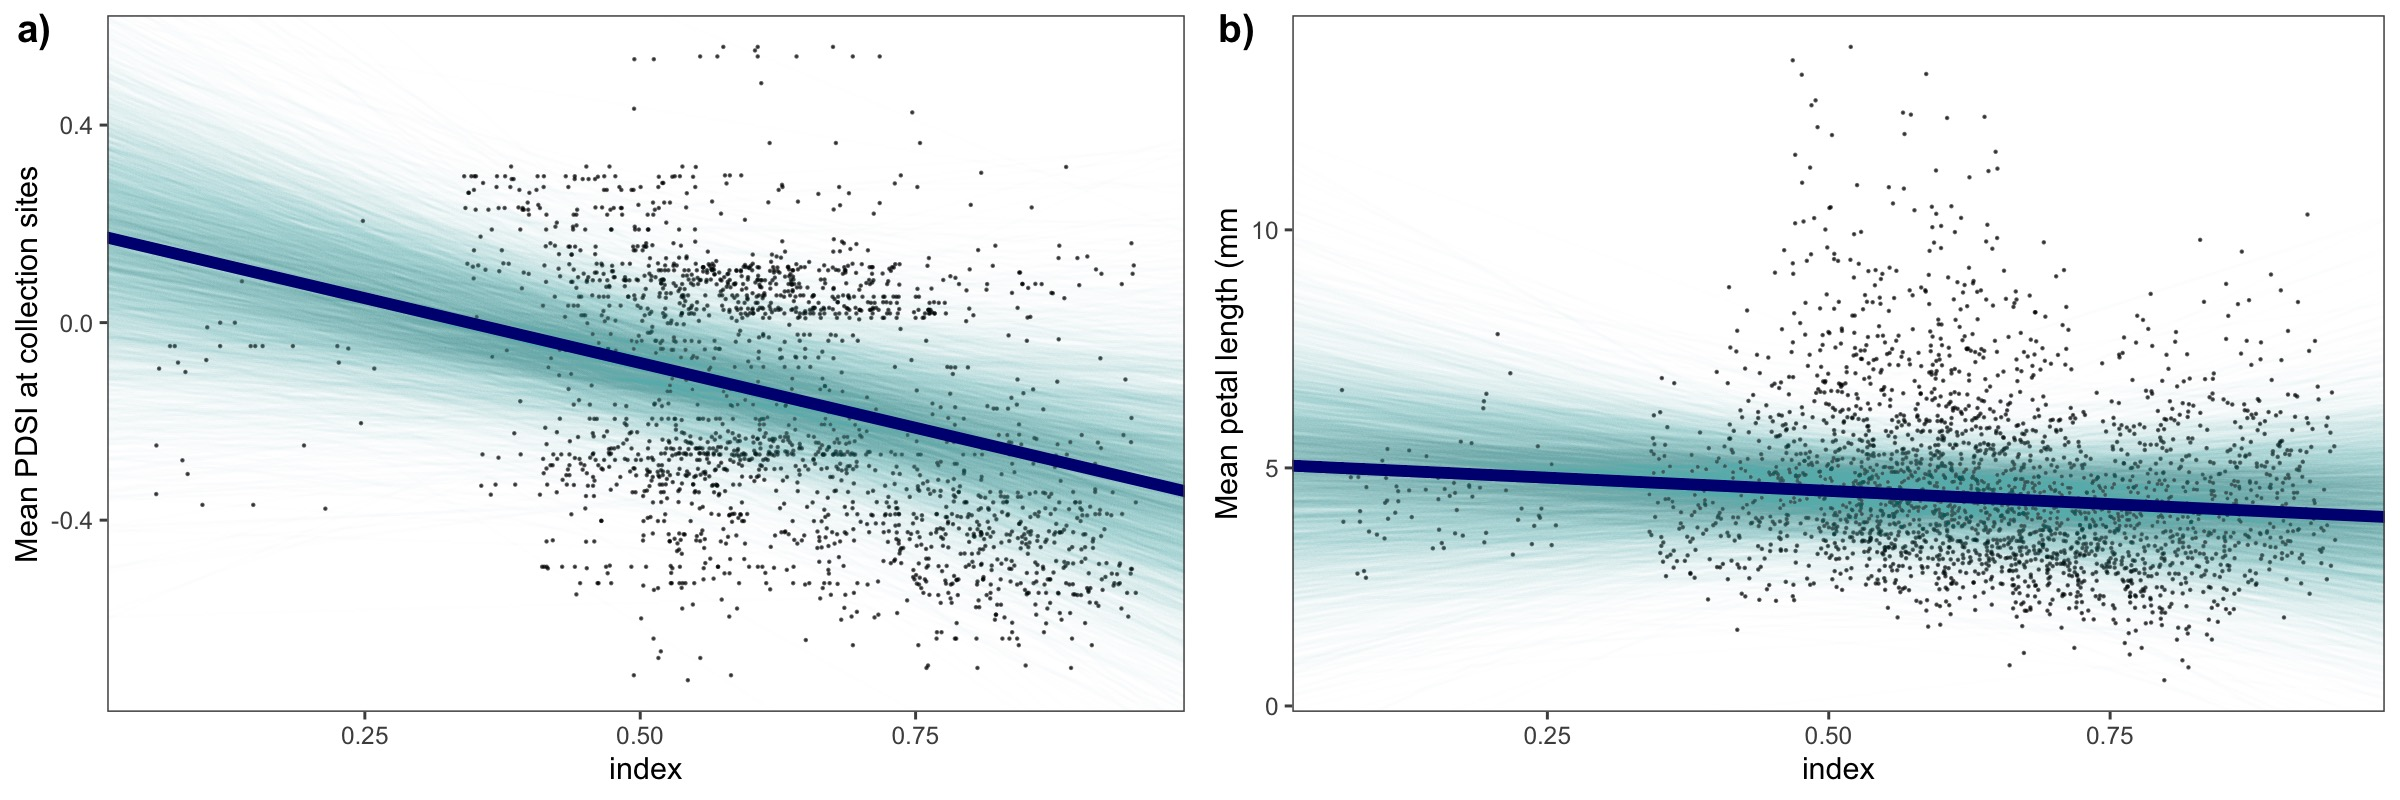
\includegraphics[width=.95\textwidth]{..//..//Plots/dataplots_SUPP.jpeg}
    \caption{Relationships between the hysteranthy index scores and environmental and biological traits based on Bayesian phylogenetic mixed models where the relationship between hysteranthy score and PDSI a)  and mean petal length b)  were each modeled separately. Solid lines indicate the mean posterior estimate and shaded areas 4000 draws from the posterior distribution as a display of uncertainty. The points and bars represent the mean estimate and standard error for each species. These plots complements the model presented in Fig. \ref{fig:prunes}}
    \label{fig:seps}
\end{figure}

\begin{figure}[h!]
    \centering
 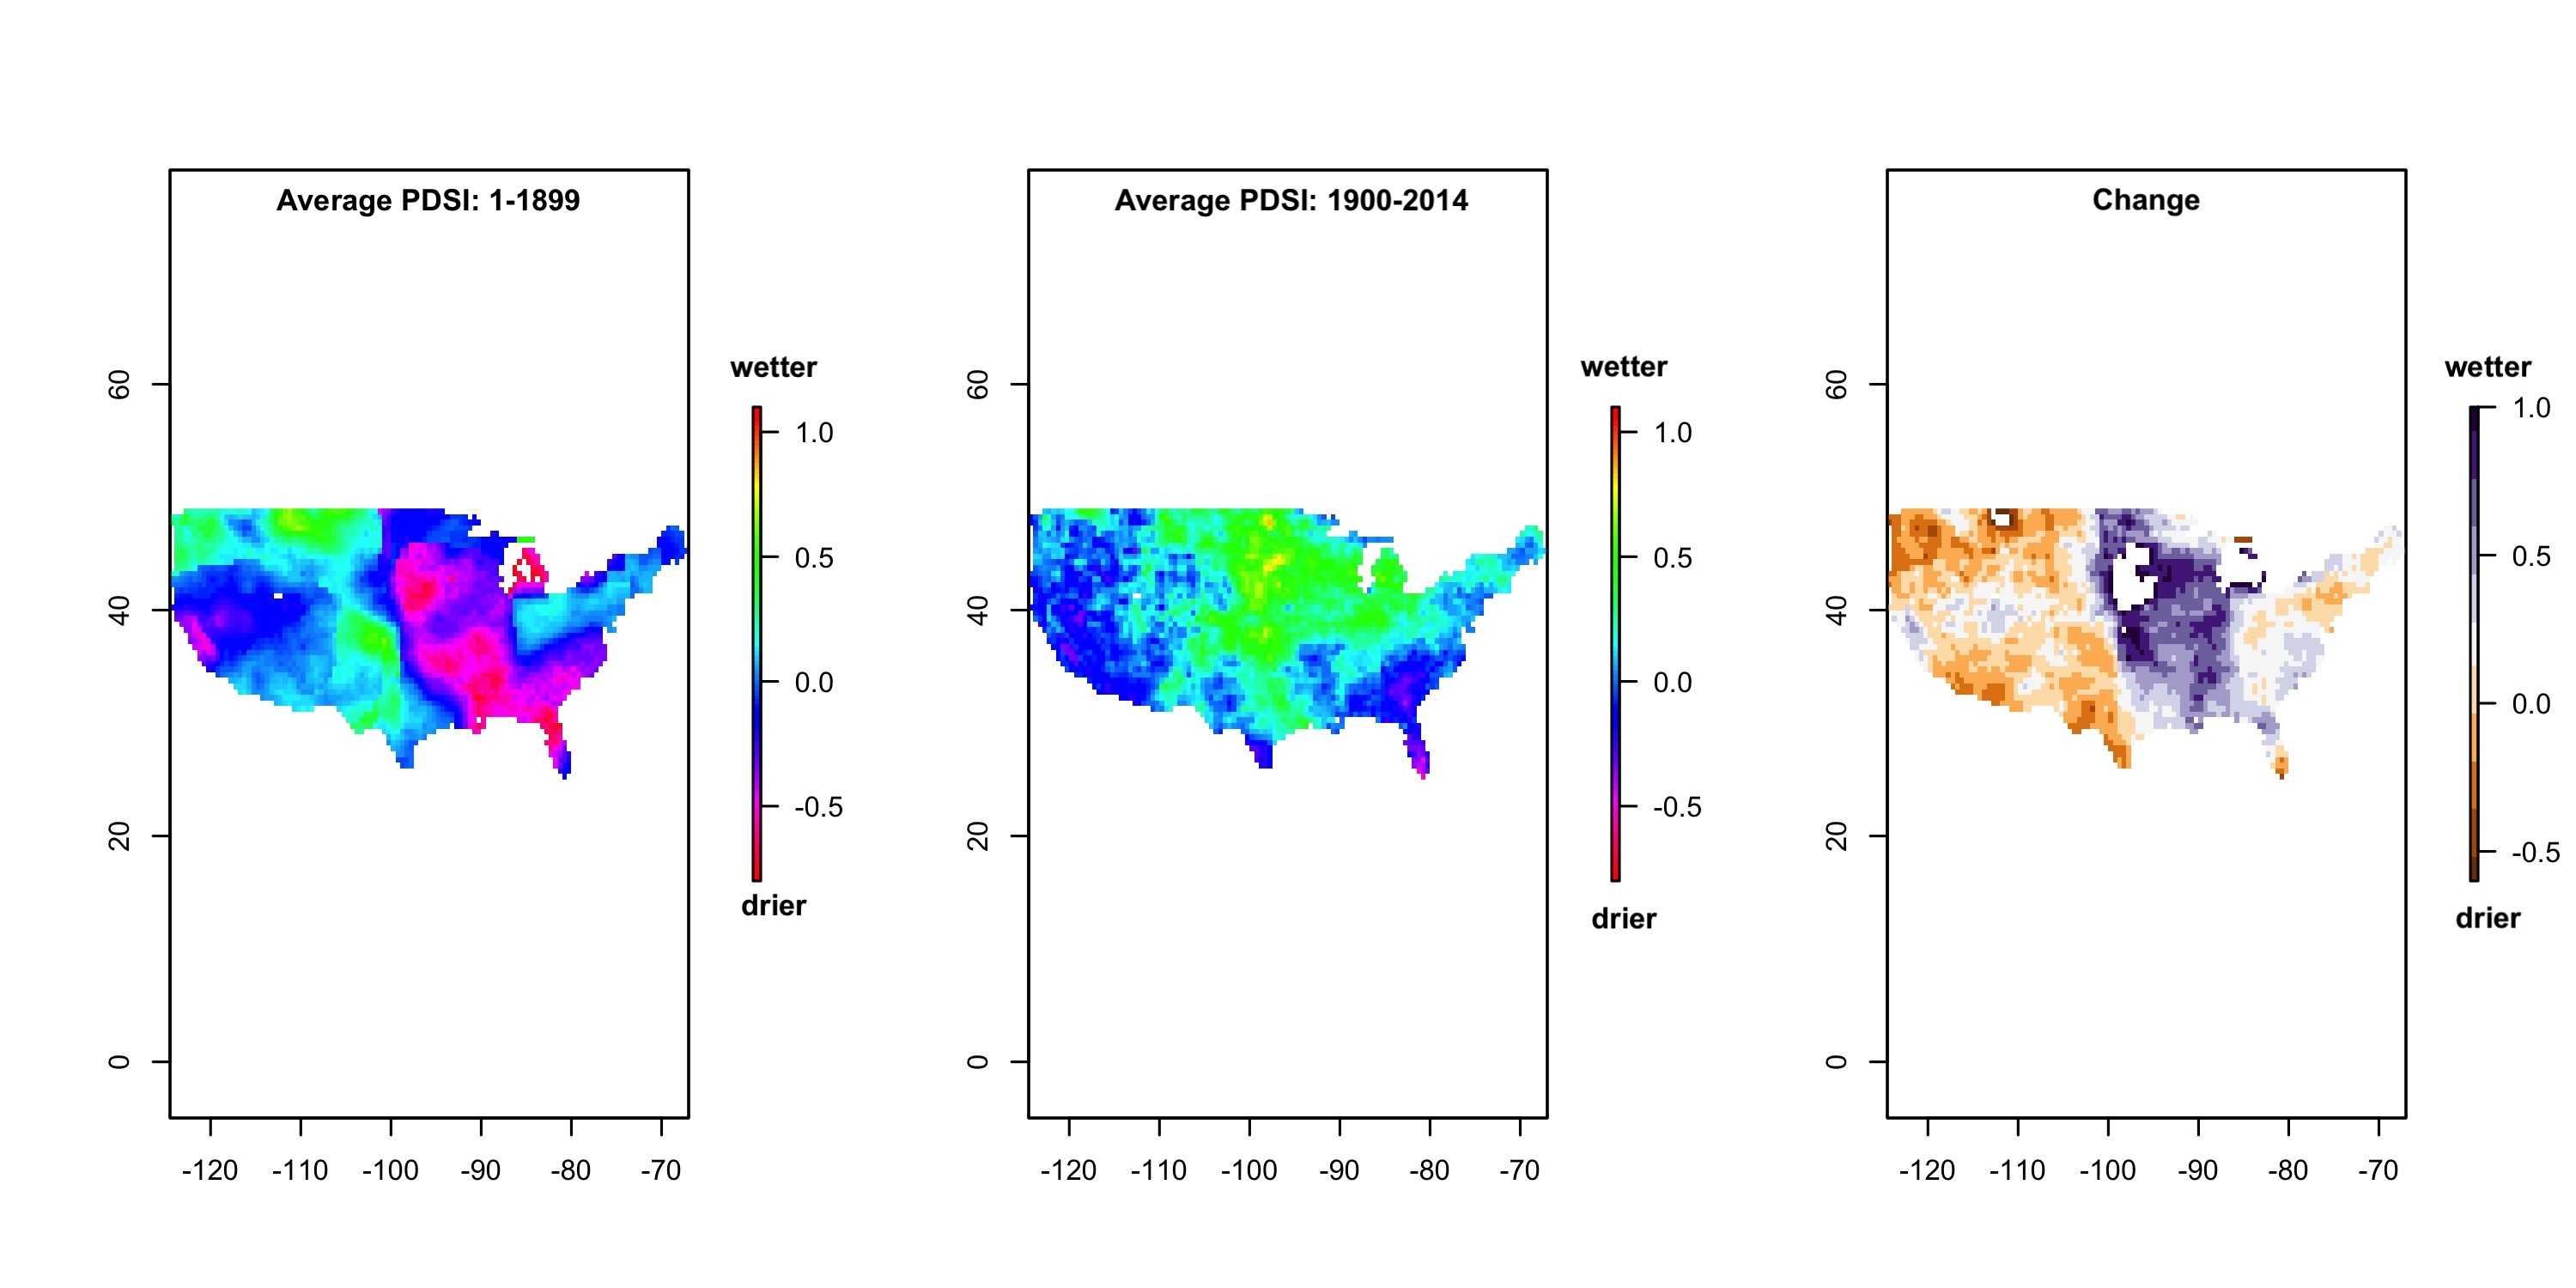
\includegraphics[width=\textwidth]{..//..//Plots/PDSIovertimemaps.jpeg}
    \caption{Average PDSI values for two time periods and the difference between them across the contiguous United States. The data used here are from \citet{Gile_2017}, and show that the south-central United States, which encompasses the ranges of many species in this study (see Fig. \ref{fig:phylo2}), has gotten considerably wetter in the contemporary period.}
    \label{fig:timeschange}
\end{figure}

\pagebreak

\section*{Extended Methods:}
To complement our main analyses in which we fit models based on species-level means of PDSI and petal length as predictors, we also implemented additional models where we assessed the relationship between PDSI and hysteranthy, and the relationship between petal length and hysteranthy separately. With this model structure our analyses accounted for the intra-specific variation in both PDSI and petal length as the phylogenetic structure of these variables.

 In these models, we modeled species and phylogeny as in the main text.
The model structure is: 

  $y_{trait} &= \alpha +\alpha_{sp} +\alpha_{phylo} + \beta_{hyst.index}*X_{hyst.index} + \epsilon$\\
  
  \epsilon & \sim N(0,\sigma^2_y) \\ %Check this
  
  where $y_{trait}$ is observed trait values (PDSI or petal length), and the slope $\beta_{\text{hyst.index}$ describes the relationship between extended hysteranthy (higher hysteranthy index value) and the trait of interest. $\alpha$ describes a grand intercept, and $\alpha_{sp}$ and $\alpha_{phylo}$ describe the species and phylogenetic effects respectively. 

\pagebreak

\bibliography{refs/hyst_outline.bib} 

\end{document}
